\documentclass[border=4pt]{standalone}
\usepackage{tikz}
\usetikzlibrary{arrows.meta,positioning,fit,backgrounds}
\definecolor{boxblue}{RGB}{225,238,252}
\definecolor{boxgreen}{RGB}{225,247,231}
\definecolor{boxorange}{RGB}{253,236,216}
\definecolor{boxgray}{RGB}{237,237,237}
\definecolor{boxred}{RGB}{253,226,226}
\begin{document}
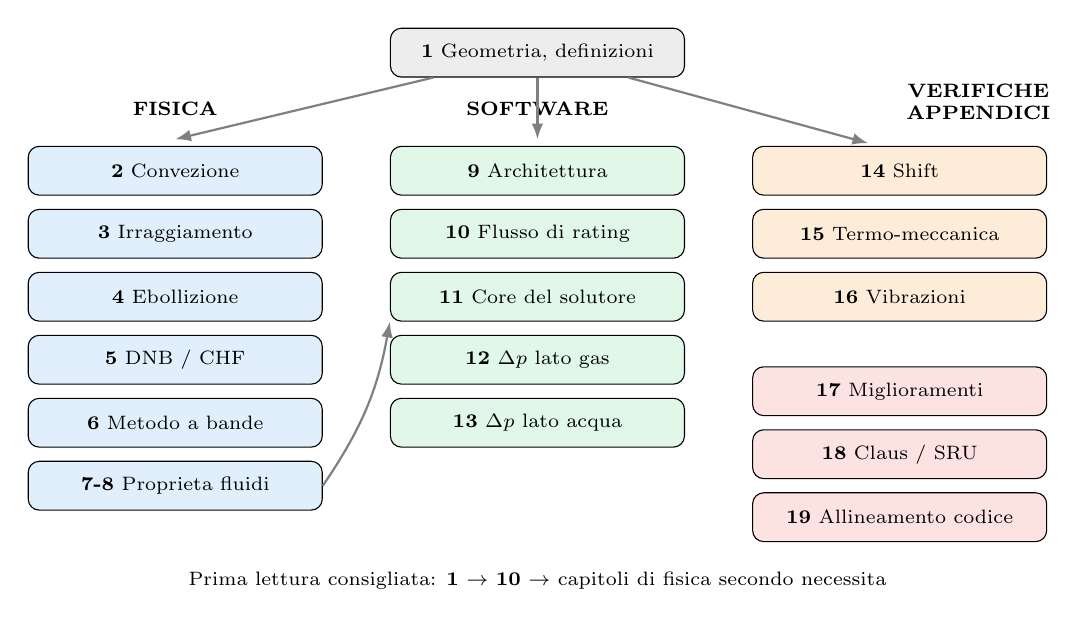
\begin{tikzpicture}[
  ch/.style={draw, rectangle, rounded corners, minimum height=0.62cm, text width=3.5cm, align=center, font=\scriptsize},
  grp/.style={draw, rounded corners, inner sep=6pt, dashed},
  arr/.style={-{Latex[length=2mm]}, thick, gray}
]
% Fondamenta
\node[ch, fill=boxgray] (c1) at (0,0) {\textbf{1} Geometria, definizioni};
% Fisica
\node[ch, fill=boxblue] (c2) at (-4.6,-1.5) {\textbf{2} Convezione};
\node[ch, fill=boxblue] (c3) at (-4.6,-2.3) {\textbf{3} Irraggiamento};
\node[ch, fill=boxblue] (c4) at (-4.6,-3.1) {\textbf{4} Ebollizione};
\node[ch, fill=boxblue] (c5) at (-4.6,-3.9) {\textbf{5} DNB / CHF};
\node[ch, fill=boxblue] (c6) at (-4.6,-4.7) {\textbf{6} Metodo a bande};
\node[ch, fill=boxblue] (c7) at (-4.6,-5.5) {\textbf{7-8} Proprieta fluidi};
% Software
\node[ch, fill=boxgreen] (c9) at (0,-1.5) {\textbf{9} Architettura};
\node[ch, fill=boxgreen] (c10) at (0,-2.3) {\textbf{10} Flusso di rating};
\node[ch, fill=boxgreen] (c11) at (0,-3.1) {\textbf{11} Core del solutore};
\node[ch, fill=boxgreen] (c12) at (0,-3.9) {\textbf{12} $\Delta p$ lato gas};
\node[ch, fill=boxgreen] (c13) at (0,-4.7) {\textbf{13} $\Delta p$ lato acqua};
% Verifiche
\node[ch, fill=boxorange] (c14) at (4.6,-1.5) {\textbf{14} Shift};
\node[ch, fill=boxorange] (c15) at (4.6,-2.3) {\textbf{15} Termo-meccanica};
\node[ch, fill=boxorange] (c16) at (4.6,-3.1) {\textbf{16} Vibrazioni};
% Appendici
\node[ch, fill=boxred] (c17) at (4.6,-4.3) {\textbf{17} Miglioramenti};
\node[ch, fill=boxred] (c18) at (4.6,-5.1) {\textbf{18} Claus / SRU};
\node[ch, fill=boxred] (c19) at (4.6,-5.9) {\textbf{19} Allineamento codice};

\node[font=\scriptsize\bfseries] at (-4.6,-0.72) {FISICA};
\node[font=\scriptsize\bfseries] at (0,-0.72) {SOFTWARE};
\node[font=\scriptsize\bfseries,align=center] at (5.6,-0.62) {VERIFICHE\\ APPENDICI};

\draw[arr] (c1) -- (-4.6,-1.1);
\draw[arr] (c1) -- (0,-1.1);
\draw[arr] (c1) -- (4.2,-1.15);
\draw[arr] (c7.east) to[bend right=12] (c11.south west);
\node[font=\scriptsize, align=center] at (0,-6.7) {Prima lettura consigliata: \textbf{1} $\rightarrow$ \textbf{10} $\rightarrow$ capitoli di fisica secondo necessita};
\end{tikzpicture}
\end{document}
